\documentclass[11pt]{article}

% Default margins are too wide all the way around. I reset them here

\usepackage[a4paper,
			twoside,
			left=1.5in,
			right=1.0in,
			textheight=9in, 
			headheight=14pt]{geometry}
			
\usepackage[utf8]{inputenc}
\usepackage[T1]{fontenc}
\usepackage{lmodern}
\usepackage[danish,english]{babel}
\usepackage{setspace}
\usepackage[pdfborder={0 0 0}]{hyperref}

\usepackage{amsmath}
\usepackage{amsfonts}
\usepackage{amssymb}
\usepackage{graphicx}
\usepackage{csquotes}
\usepackage{appendix}
\usepackage[backend=biber, style=apa, sorting=nyt]{biblatex}
\usepackage{algorithm}
\usepackage{algorithmic}
\usepackage{subfigure}
\usepackage{fancyhdr}
\usepackage[labelfont=bf]{caption}
\usepackage{listings}
\usepackage[usenames,dvipsnames,table]{xcolor}

\colorlet{NotLavender}{Lavender!30}
\colorlet{NotGreenYellow}{GreenYellow!30}
\colorlet{NotSkyBlue}{SkyBlue!20}
\colorlet{NotOrange}{Orange!20}
\colorlet{NotRed}{Red!30}
\colorlet{NotGreen}{Green!20}
\colorlet{NotPurple}{Purple!20}

\definecolor{DarkGreen}{rgb}{0.0,0.4,0.0}
\definecolor{highlight}{RGB}{255,251,204}
\renewcommand{\lstlistingname}{Snippet}
\lstset{language=C++, 
		basicstyle=\footnotesize, 
		breaklines=true, 
		breakatwhitespace=false, 
		keywordstyle=\bf\color{Blue},
		firstnumber=1,
		frame=lines,
		numbers=left,
		numbersep=10pt,
		numberstyle=\tiny\color{Gray},
		stepnumber=5,
		stringstyle=\color{Purple},
		commentstyle=\usefont{T1}{pcr}{m}{sl}\color{DarkGreen},
		captionpos=b
}

\DeclareLanguageMapping{english}{english-apa}
\graphicspath{{images/}}
\addbibresource{bib.bib}


\author{Group 514}
\title{Report}

%\includeonly{./chapters/introduction}

\begin{document}

%------------------------------------------------------------------------------
% TITLE
%------------------------------------------------------------------------------
\fancyhf{}
\pagestyle{plain}
\pagenumbering{roman}

\section*{Readers Guide} \label{sec:readersguide}
\section*{Glossary} \label{sec:glossary}

\maketitle
\setcounter{tocdepth}{2}
\tableofcontents

\clearpage
%------------------------------------------------------------------------------
% CONTENT
%------------------------------------------------------------------------------
\setstretch{1.3}
\pagestyle{fancy}
\renewcommand{\sectionmark}[1]{\markboth{#1}{}}
\fancyhead[RE, LO]{Chapter \thesection . \emph{\nouppercase{\leftmark}}}
\fancyhead[RO, LE]{\thepage}
\pagenumbering{arabic}

%!TEX root = ../main.tex
\section{Introduction} \label{sec:introduction}
Artificial intelligence is a growing market and have been for a long time. Whether it is security systems, the stock market or video games, there is always a need for better AI?s capable of doing calculations better than humans or to mimic human behaviour more accurately. The recent years a specific form of AI?s called Evolutionary Algorithms have seen more application, and are used in a wide range of programs. The concept has been around for many years, but it is only with modern computing capacity that we are able to apply these algorithms in more demanding programs to do more advanced tasks. An evolutionary algorithm (EA) mimics the rules and laws of natural selection for the sake of optimization, where the fittest individuals in a population forms new generations, ideally becoming ?stronger and stronger?. Obviously this is in very general terms. EA?s do not have to evolve a species or civilization. It can for instance also be used to create a perfect wing for an airplane given the right parameters, or calculate the shortest route between multiple cities, as is the case in the famous Travelling Salesman example. 

Meanwhile, in the video games industry, a subset of EA?s called Genetic Algorithms (GA) are being experimentet with as well. Especially in terms of balancing systems, and creating adaptive AI opponents, such as in strategy games which have many different parameters that have to be balanced. For instance making sure that one army is not stronger than another but still have different units and abilities. Genetic algorithms are perfect for these kinds of optimizations, for finding the most optimal configuration, where testing every possible configuration manually to get the most balanced result would otherwise take weeks, months, years etc. EA?s and GA?s are all about feeding an algorithm the right parameters and then evaluating the individuals/solutions correctly to achieve a better and better solution for each generation the algorithm evolves.

In this project we have chosen to implement a genetic algorithm in Pac-Man to see how this would alter the behaviours of the ghosts/monsters in the game. Pac-Man has been used as a base for GA experimentation before, as these older games seem to lend themselves well by having relatively simple programming and non-costly performance cost on the system. The goal for this project is to see if the GA can make the game increasingly more difficult by utilizing this type of algorithm for the AI of the ghosts i.e. does the GA evolve the ghosts according to our expectations of the outcome of the fitness evaluation of the algorithm.


\subsection{Initial Problem Statement} \label{sec:initialproblemstatement}
Is it possible to create an artificial intelligence video game opponent, which modifies itself according to the players' performance?

%!TEX root = ../main.tex

\section{Investigation} \label{sec:preanalysus}
This chapter will investigate and discuss the viability of the initial problem statement from above. It will the investigate the various aspects of artificial inteligence as well as state of the art within self-modifying AIs. The chapter will also provide various delimitations as to which parts of the initial problem statement can be used for further analysis. This chapter will develop the initial problem statement into a final problem statement.




%!TEX root = ../../main.tex


\subsection{Artificial Intelligence} \label{sec:ai}
Artificial Intelligence (AI) has been, and is still one of the absolute big buzzword in the science industry.
The idea of giving a machine, human characteristics have been around for centuries and is still a field that demands a lot of attention, \cite {Buchanan2006} nevertheless is successful, \cite {Franz2014} \cite {Varkey2014} and have therefor become a constantly growing field for each time it is proven possible. (XX Kilde)

One field with great success is the gaming industry, who have found AI as a good entertainment source in commercial games when developing a NPC opponent. (XX kilde)   An NPC is a game character (or several characters) there is not controlled by a person but by the computer. \cite {Definition2014}  For example have a NPC recently been developed to train medical and military students in real life high-risk situations through a educational application. (XX Kilde)

As the name Artificial Intelligence implies can the term AI have several meanings. It may refer to different areas of specialization such as games playing, expert systems, natural language, neural networks and robotics. \cite {Vangie2014}
Therefor whenever we further use the term AI in this report, are we referring to the idea of incorporating a game opponent (NPC) as opposed to a mechanical AI.



\subsubsection{Definition of AI}

Although numerous definitions already exist, would we still like to define what we consider an AI. Our general definition will follow the Oxford dictionaries and be defined thus:

		\begin{quote}
		The theory and development of computer systems able to perform tasks normally requiring human 		intelligence, such as visual perception, speech recognition, decision-making, and translation between languages. \cite {Oxford2014}
		\end{quote}

However as stated earlier will we not investigate fields such as speech recognition, translation or visual perception. Therefore will we further break down the general definition and look at the exact meaning of AI's two former arguments, Artificial and Intelligence.

We have adopted the official definition of Artificial, which state artificial is not necessarily associated with computers and technology. \cite {artificial2014} It just means something biological has been made by humans, imitated a natural origin and produced a copy of it.

In gaming AI are we considering artificial an imitation of the human brain. The brain is the main component because this is were humans store personality, self-awareness and control self-operating actions, which is what scientist would like to modernize to mechanics. (XX Kilde)
Keep in mind that we do not see self-operating as the same as self-awareness. According to game developer Kehoe, 2009 should a gameplay should not possess this action. \cite {Kehoe2009}Gameplays is perceived as a form of entertainment and should therefor not be aware of anything beyond the scope. The purpose of the AI is to simulate a intelligent behavior that gives the opponent a believable challenge that can be overcome.

But what is intelligent behavior? Intelligence is hard to define since it does not have a solid definition that can characterize what kinds of computational procedures we want to call intelligent.  \cite {McCarthy2007} Therefore in our case is intelligence defined as the ability to achieve fixed goals out from several observations.
It should base its observation out from the trial and error method, trying out random moves until one is found succesful and store that information until next time the AI is placed in same problem.

All this put together is what we call an intelligent Agent (IA).

"An agent is anything that is capable of acting upon information it perceives. An intelligent agent is an agent capable of making decisions about how it acts based on experience. An autonomous intelligent agent is an intelligent agent that is free to choose between different actions. "  \cite {Mills2005}



\subsubsection{General types of AI's in games}

As we state in our IPS are we researching the possibility in creating an AI that modifies itself according to players' performance. We find that it is not relevant to investigate AI behavior that can not alter itself in a adaptive manner as we are looking for. For this are we not looking further into General AI in games.


\subsubsection{Self-modifying artificial intelligence in games}
\label{section:selfmodifyingai}

In order to establish knowledge as to what type of artificial intelligence can be modified, and how, the term of "self modifiable" artificial intelligence must be elaborated. We must therefore find examples and pre-existing theories of AI systems in games that is able to alter it's predefined set of behaviours through some adaptive algorithms as a sort of self modification.

As described by Booker et al, 2005 \cite{Booker2005} in a revised perspective of the work on adaptations in natural and artificial systems conducted by John Holland, it is defined that systems that utilizes behaviours such as learning or adaptation is known as complex adaptive systems(CAS).\cite[pp. 1]{Booker2005}

It is mentioned that such systems is able to change behaviours in response to the surrounding environment while also being capable of changing the rules that actually controls it's own behaviour through learning.

Complex adaptive systems, as described by Booker et al, is a growing subject of research within the field of biological inspired computing\cite{Booker2005} . Systems imitate some CAS in nature in order to solve computational problems, which is the process of conducting calculations through computer technology. They describe the following examples of biological computing aspects to be of interest within the development of CAS:

	\begin{itemize}
	\item Evolutionary Computation
	\item Neural computation
	\item Ant-Colony-inspired algorithms
	\item Immune-system
	\item Computer security
	\item Molecular Computing
	 \end{itemize}

Lansing, 2003 \cite{Lansing2003} validates that CAS are research within the fields of social sciences along with natural sciences.  The following aspects of the mentioned CAS are however only of relevance if the mentioned examples are somewhat applicable, in any way, to artificial intelligence aspects in games.\\
Of great interest and relevance lies the aspects and usability of evolutionary computation. Evolutionary computation is the method of constructing problem solving systems, which does so by the use of computational evolutionary models.\cite{Howe2010} Amongst the plausible models of evolutionary computation lies evolutionary algorithms, genetic algorithms, evolution strategies, evolutionary programming and artificial life\cite{Howe2010}\\

Lucas and Kendall, 2006 \cite{Lucas2006} describes how evolutionary computational intelligence can be applied in games as they provide  \enquote{ competitive, dynamic
environments that make ideal test beds
for computational intelligence theories,
architectures, and algorithms.}\cite[pp. 10]{Lucas2006}\\
Examples of implemented evolutionary computation in both board games and video games is concluded to, in some cases, be superior to other systems. They describe how evolutionary computation is applicable in games and mention the development of new game genres based upon evolutionary computation. Additionally, while refering to 2D arcade game of Pacman, they describe that \enquote{advantage
of working with older-style arcade games is that they
offer a sufficiently interesting challenge, while being much
easier to implement and faster to simulate.} \cite[pp 15]{Lucas2006} \\

As Lucas and Kendall has validated the usage of Pacman as a possible test bed for evolutionary computation, the relevance of examining pre existing implementations, using Pacman, is self apparent.\\
As mentioned earlier, evolutionary computation offers several models of computation. By examining the existing implementations, we can most likely distinguish one or several methods of successfully implementing evolutionary computation.

\subsubsection{Evolutionary computation in Pacman}


There exists many examples of applied evolutionary algorithms in Pacman, as well as Ms. Pacman whereof the earliest examples was that of Koza in 1992.\cite{Koza1992}

This implementation utilized genetic programming and was aimed at controlling Pac-Man himself through functions, conditions and primitives to evolve the movement of Pac-Man. \cite[pp. 2]{Lucas2005}
Research conducted by Simon M. Lucas in 2005 also tried to approach a method to evolve Ms. Pac-Man playing agents through the use of an evolutionary algorithm. \cite{Lucas2005}

With their evolutionary algorithm the objective was to evolve the best possible player, where they measured some average score over numerous games, in order to create a neural network to be evolved. \cite[pp. 8]{Lucas2005}

in the conclusions of their research, it is mentioned that whether or not the ghosts behaved deterministic or non-deterministic would have a significant effect on the evolved player. A non-deterministic version of the game would result in a much harder game  as the evolved player must learn strategies under different circumstances in the game rather than exploiting the deterministic game, where the game would have a certain way the ghosts move, which would become predictable for the evolved player.\cite[pp. 8]{Lucas2005}

Much similarly, but with the focus on ghost behaviour, is the research of Kalyanpur and Simon, 2001. They propose a method to improve the level of play of the ghosts in Pacman by the use of an evolutionary computation method that utilized a combination of genetic algorithms and neural networks. \cite{Kalyanpur2001}

amongst the conclusions of their implemented Genetic Algorithm and Neural Networks, they describe that it can indeed be applied in games such as Pacman. Additionally they describe the Genetic Algorithms are used to isolate the best strategy, represented by the fittest ghosts of a current generation of ghosts, and thereby pursue to include these characteristics of ghost behaviour onto the next generation. \cite[pp. 8]{Kalyanpur2001}

The implemented Neural Network is described to calculate the Genetic Algorithm parameters, which is used to improve the actual efficiency of their mentioned genetic reproduction within the game. Generally for the conclusions of their implementation is that there indeed is potential in the usage of evolutionary computation in games.

It is however noteworthy that their Pac-Man platform is self constructed, and does not use the original game platform as a test bed for the research in ghost behaviour.

An example of implemented Genetic Programming is also done by Brandstetter and Ahmadi, 2012. They propose an approach as to how Ms. Pacman can be controlled based on a Genetic Algorithm.
They describe how Ms. Pac Man can be controlled by retrieving information about the current game state in order to find some optimal movement direction.
With their applied method of application, the evolved Ms. Pac Man controller was able to play on a level of a good beginner human player. \cite{Brandstetter2012}

The mentioned examples are a few possible implementations of evolutionary computation in Pacman and Ms. Pacman. The combined applied methods in these examples are genetic programming, genetic algorithms, neural networks to control genetic algorithm parameters and evolutionary algorithms.\\

The difference between genetic algorithms and genetic programming is the actual representation of solutions, whereof the genetic programming is a subsection of genetic algorithms. The algorithm creates strings of data that combined represent some solution to a problem and the programming solutions are actual computer programs.\cite{genetic}
Genetic algorithms and genetic programming are subtypes of evolutionary algorithms.

What is interesting about the examples of applied evolutionary computation in Pacman is the method of application. The implementation does solely focus upon the improved solutions of the actual behaviours of either the ghost(s) or Pacman AI.\\
Even though a prominent factor of Pacman AI is the behaviour of either the ghosts or Pacman, there are certain aspects which is still not speicified in the above mentioned examples of evolutionary computation implementation. Behaviours of either the ghosts or pacman is described, but there are several other aspects of plausible application of evolutionary computation that serves as a interesting aspect of plausible application of evolutionary computation.\\

\subsection{Artificial Intelligence in Pacman(SOTA)}
%!TEX root = ../../main.tex

\subsubsection{Original AI modes}
The four enemies in Pac-Man may appear to move in a random fashion but each of the four ghosts actually move in a deterministic fashion~\autocite{Pittman2011} They all share the same behavior modes that they can switch between; \textbf{Chase}, \textbf{scatter}, and \textbf{frightened} mode.

\emph{Chase mode} is, in all its simplicity, about chasing the Pac-Man down through the maze.

In \emph{scatter mode}, the ghosts forgets the Pac-Man and heads to their corner of the maze. This mode is only be active for a few seconds before they revert to chase mode.

When the Pac-Man eats one of the four special pellets in the maze, the ghosts go into \emph{frightened mode}. In Frightened mode, the ghosts will turn dark blue, turn around and aimlessly wander the maze for a few seconds before they return to their previous mode. In frightened mode the ghosts become vulnerable (indicated by the dark blue color) and it is possible for the Pac-Man to eat the ghosts for extra points. When a ghost is eaten it will return to the box in the middle of the maze as well as resume its previous mode.

The effects of frightened mode is different depending on how far in the game the player is; as the levels progress the time spend in fright mode is shortened until they no longer become frightened (They still lose their target and wander aimlessly).

These modes are part of what is called a finite state machine~\autocite[pp.44]{Buckland2005}~\autocite{Kehoe2009}.
A finite state machine is one of the most basic concepts in video game AI programming. The machine consists of a finite set of fixed states that it can occupy(In the case of a light switch those states would be ON and OFF) at any given moment in time. It can be difined like this:

\blockquote[\autocite{Buckland2005}]{\enquote{A finite state machine is a device, or a model of a device, which has a finite number of states it can be in at any given time and can operate on input to either make transitions from one state to another or to cause an output or action to take place. A finite state machine can only be in one state at any moment in time.}}

The finite states in Pac-Man are the modes mentioned above and the transition between these modes~\autocite[pp.45]{Buckland2005}.
\subsubsection{Self-modifying AI's in Pacman / Ms. Pacman}

Contrary to the classic arcade Pacman, where the implemented AI is provided as a fixed set of behaviours within the game, regardless of player performance, a self modifying AI would take some parameters into account and apply some continuous optimization. This method of applying some sort of optimization is known as evolutionary computation.


There exists many examples of applied evolutionary algorithms in Pacman, as well as Ms. Pacman whereof the earliest examples was that of Koza in 1992.\cite{Koza1992}

This implementation of genetic programming was aimed at controlling Pac-Man himself through functions, conditions and primitives to evolve the movement of Pac-Man. \cite[pp. 2]{Lucas2005}
Research conducted by Simon M. Lucas in 2005 also tried to approach a method to evolve Ms. Pac-Man playing agents through the use of an evolutionary algorithm. \cite{Lucas2005}

With their evolutionary algorithm the objective was to evolve the best possible player, where they measured some average score over numerous games, in order to create a neural network to be evolved. \cite[pp. 8]{Lucas2005}

in the conclusions of their research, it is mentioned that whether or not the ghosts behaved deterministic or non-deterministic would have a significant effect on the evolved player. A non-deterministic version of the game would result in a much harder game  as the evolved player must learn strategies under different circumstances in the game rather than exploiting the deterministic game, where the game would have a certain way the ghosts move, which would become predictable for the evolved player.\cite[pp. 8]{Lucas2005}

Much similarly, but with the focus on ghost behaviour, is the research of Kalyanpur and Simon, 2001. They propose a method to improve the level of play of the ghosts in Pacman by the use of an evolutionary computation method that utilized a combination of genetic algorithms and neural networks. \cite{Kalyanpur2001}

amongst the conclusions of their implemented Genetic Algorithm and Neural Networks, they describe that it can indeed be applied in games such as Pacman. Additionally they describe the Genetic Algorithms are used to isolate the best strategy, represented by the fittest ghosts of a current generation of ghosts, and thereby pursue to include these characteristics of ghost behaviour onto the next generation. \cite[pp. 8]{Kalyanpur2001}

The implemented Neural Network is described to calculate the Genetic Algorithm parameters, which is used to improve the actual efficiency of their mentioned genetic reproduction within the game. Generally for the conclusions of their implementation is that there indeed is potential in the usage of evolutionary computation in games.

It is however noteworthy that their Pac-Man platform is self constructed, and does not use the original game platform as a test bed for the research in ghost behaviour.

An example of implemented Genetic Programming is also done by Brandstetter and Ahmadi, 2012. They propose an approach as to how Ms. Pacman can be controlled based on a Genetic Algorithm.
They describe how Ms. Pac Man can be controlled by retrieving information about the current game state in order to find some optimal movement direction.
With their applied method of application, the evolved Ms. Pac Man controller was able to play on a level of a good beginner human player.


++Insert ref til Brandstetter her. Aner ikke hvorfor det ikke fungerer++

\subsection{Summary}
We identify that GA’s had indeed been implemented in Pacman in several manners, both where Pacman and the ghosts have altered behaviours. However, we find no evident material as to how a GA implementation which self modifies the alternations between the behaviours of the opponent (ghosts) could be successfully implemented. Therefore, we see if this modification is possible, and if it does indeed have some sort of impact on the player’s performance in any plausible way.


\subsection{Final Problem Statement} \label{sec:finalproblemstatement}
Is it possible to create an implementation of a video game AI, which alternates between the various states of a finite state machine, according to the player's performance through the use of a genetic algorithm?

\section{Analysis} \label{sec:analysis}


% Pacman content research


\subsection{Pacman}
\subsubsection{AI behaviour argumentation (how they do it)}
\subsubsection{Technical details/mechanics/paramters}

\textbf{About}\\
Pacman is an arcade game which was developed by the company Namco, and was first released in 1980's.

Extensive documentation and description of Pacman has been accounted for by Pittmann, 2011 \cite{Pitmann2011}.

\textbf{Purpose}
The general purpose of the game is to control Pacman through a maze while gathering dots. Once all the dots within the maze has been collected by Pacman, the player proceeds to the next level.







\textbf{Gameplay Details}\\
The purpose of the game is to navigate Pacman though a maze by simple up,down,left,right movements to pick up small dots within the maze while avoiding being eaten by four ghost that chases the Pacman throughout the length of the game.








\subsection{Player performance}
a. Identify pacman parameters to measure player performance. (from 4.B) Associate also with  previous research(other AI implementations in Pacman. What did they use to  identify “performance”?


b. Define “good” and “bad” performance based upon 5a. (assume that we use only win/lose conditions unless prior research has based performance indications upon other game parameter results)

c. Performance results. We identify “some” performance. Therefore we configure the following “alternation of ghost behavior” in “this” way.

\subsection{Genetic Algorithm(s)}

\subsubsection{GA definitions. (what it is, and how it works}
\subsubsection{GA and Pacman(how the two can be combined.(methods)}
we must identify possible implementations of "pacman parameters" to control fitness score.

\section{List of Requirements} \label{sec:lor}

The following listed content is to be considered relevant to implement in order to answer to the final problem statement. The following list will be denoted into a bulletin order, in no particular order where the content is of importance as deemed by the group based upon research.

\subsubsection{Pacman}
\subsubsection{Genetic Algorithm}
The following content is considered to be required to construct, develop and implement a functional genetic algorithm in accordance with the final problem statement.

Sivanandam, 2008 states that the following general content is used to develop a genetic algorithm:

\enquote{\begin{enumerate}
\item The representation of the problem
\item The fitness calculation
\item Various variables and parameters involved in controlling the algorithm
\item The representation of result and the way of terminating the algorithm
\end{enumerate}} \cite[pp. 33]{Sivanandam2008}


\begin{itemize}
\item Problem definition
\item Population size.
\item Gene encoding.
\item Fitness function and Fitness Score representation
\item Selection method operator
\item Crossover operator function and crossover probability
\item Mutation operator function and mutation probability
\item result representation
\item algorithm termination

\end{itemize}


\subsubsection{Test procedure/evaluation}
\section{Methods} \label{sec:methods}
%!TEX root = ../main.tex
\section{Design} \label{sec:design}

This chapter will set focus on the research from the analysis to create a blueprint of our desired product that will fulfill the demands from our list of requirements. The prototype is going to be split into three different parts.

\begin{itemize}
\item Pacman
\item Simulation
\item Genetic Algorithm
\end{itemize}

The prototype should work as following:

New modes for the ghosts will be created that can be controlled by a finite state machine. This will create a mode cycle that will be able to be manipulated by a genetic algorithm. The goal is then to create a simulation system that can create simulations with new data sets for a fitness function to evaluate in the genetic algorithm. Then return the mode cycle that match the player’s performance for next game of pacman (See Fig. Design Plan).


\begin{figure}[!htbp]
\centering
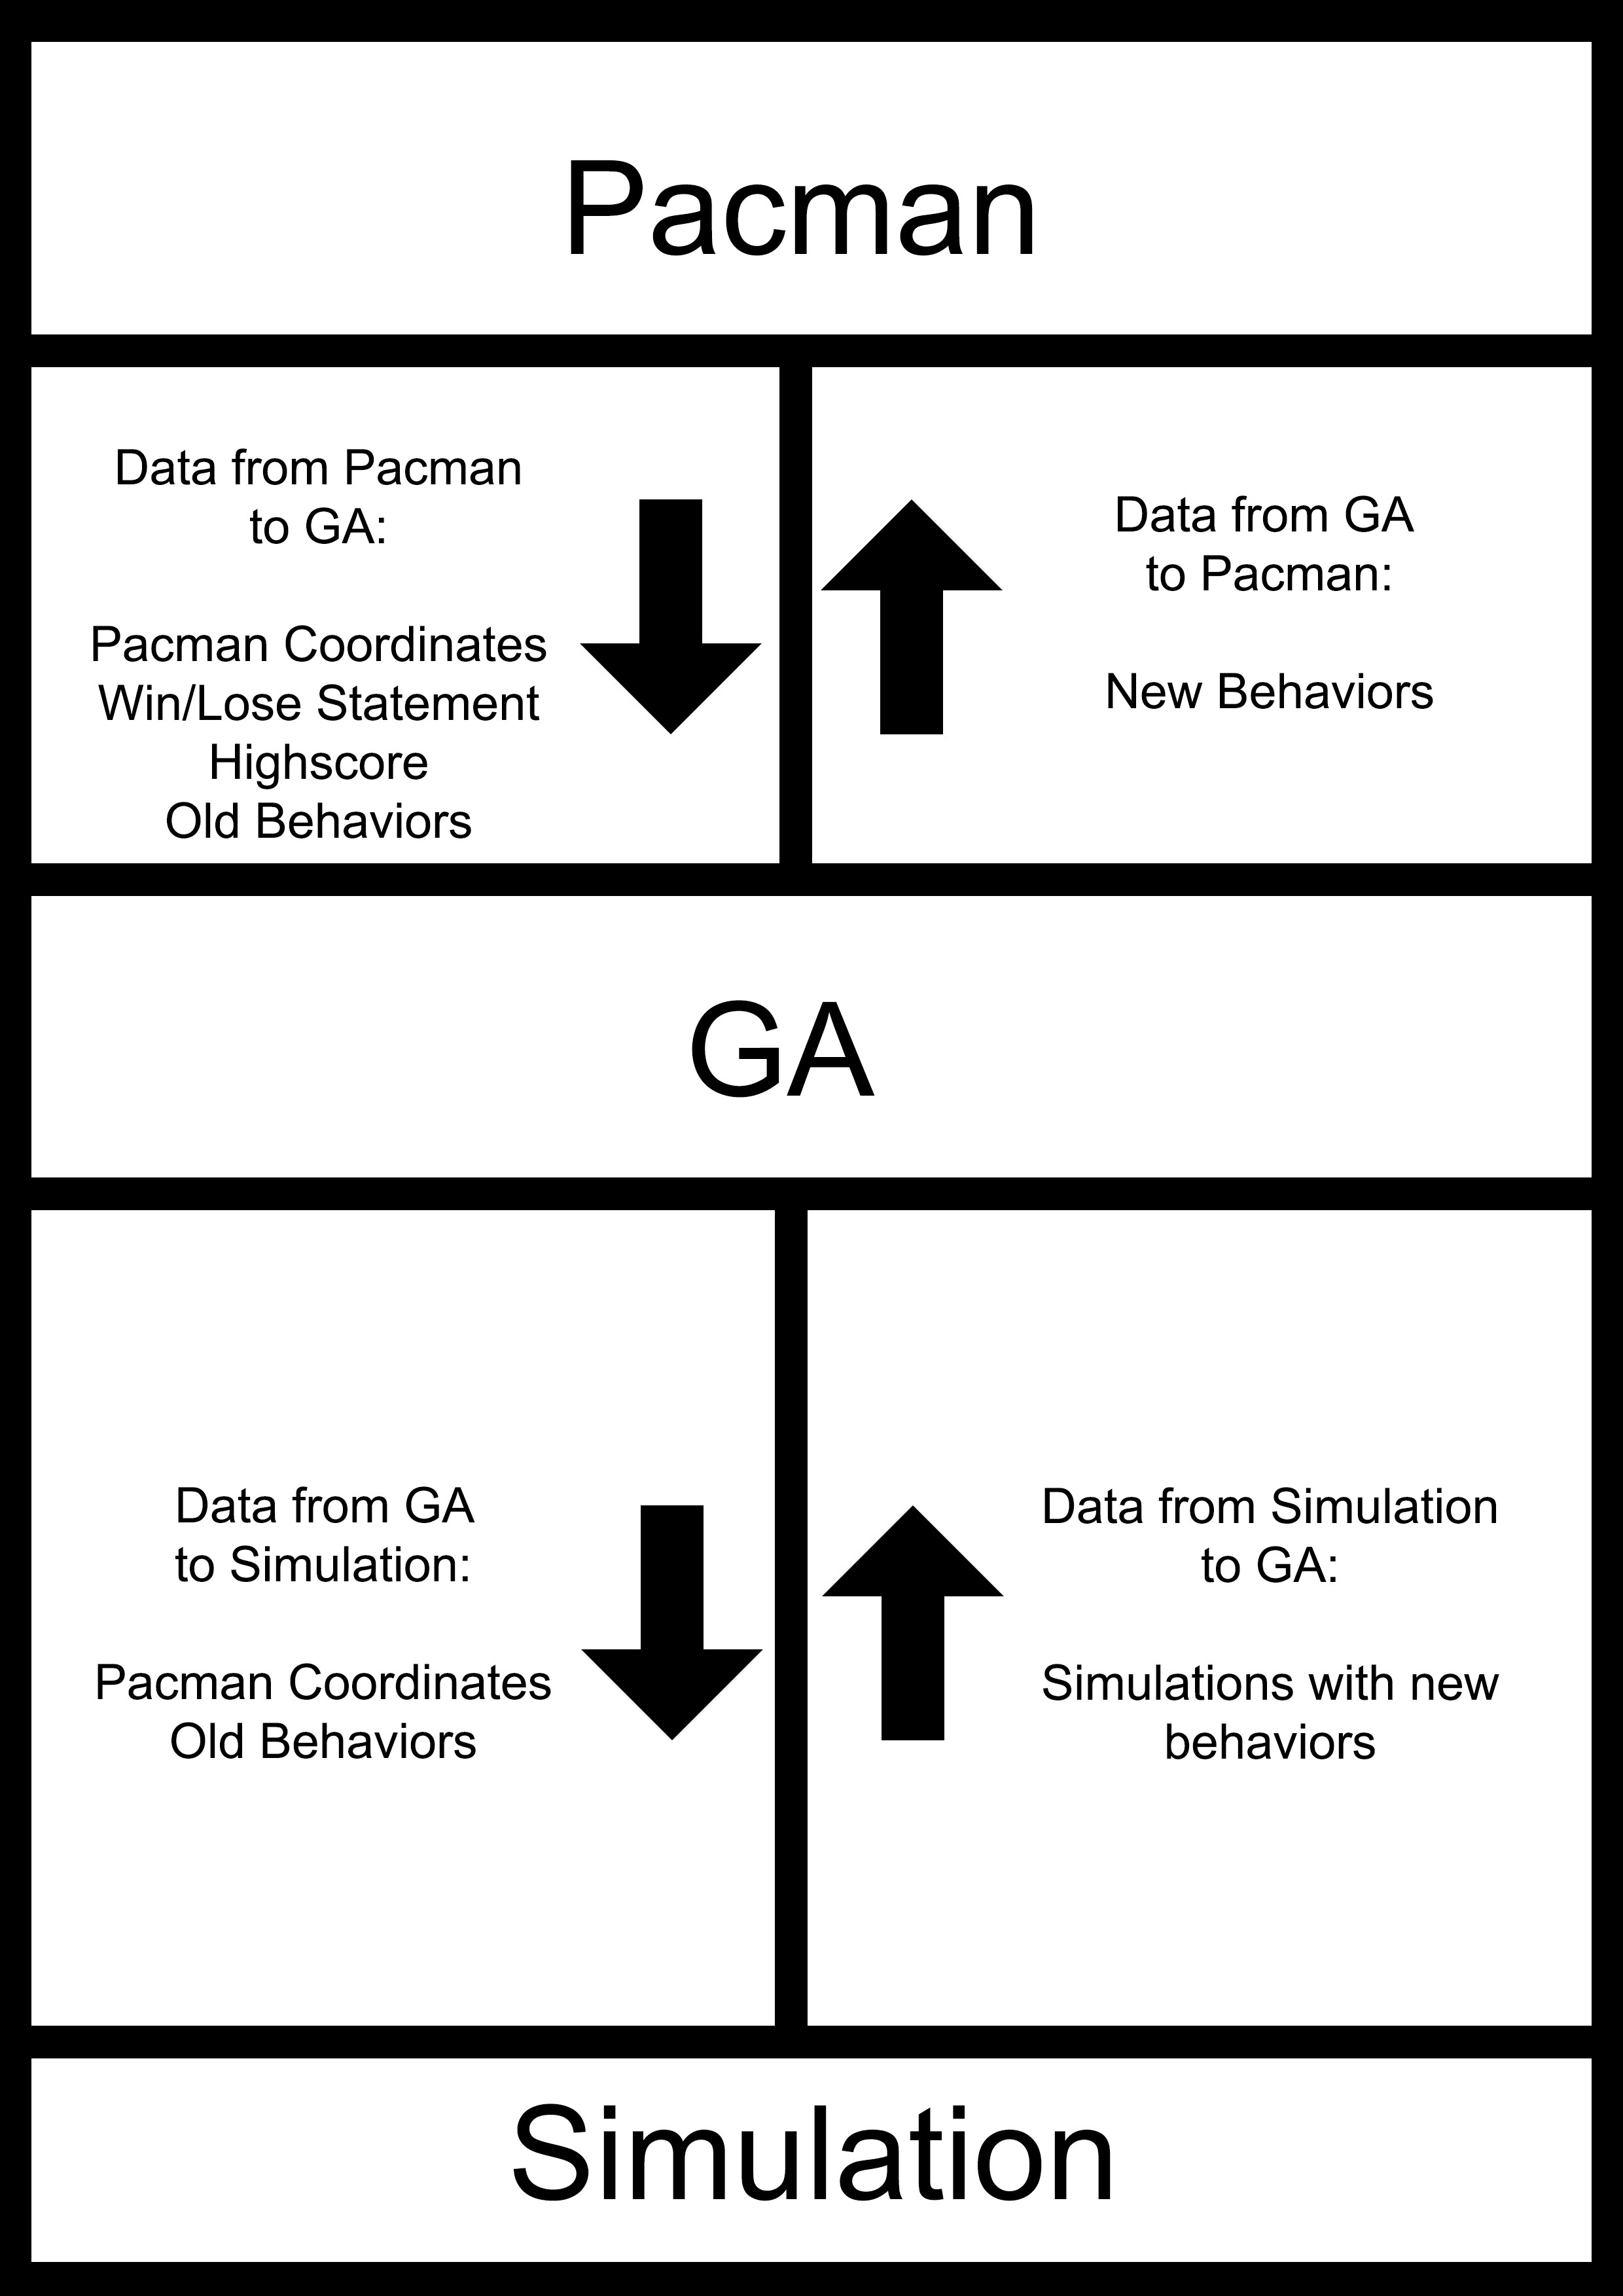
\includegraphics[width=0.5\textwidth]{D1.png}
\caption{ Design Plan }
\label{fig:DesignPlan}
\end{figure}

\subsection{Pacman Modes}\label{ssec:design_modes}

The original Pacman in its current state is not optimized for the use of a genetic algorithm. That is why it has to be tailored into a finite state machine that can be linked with the genetic algorithm and change the values that is being sent as input. We want to base this finite state machine on the different ghost modes. That means the modes are going to be switched during the gameplay and by that each ghost will no longer have a specific role in the game. An example could be that a ghost would change mode every 10 seconds or every 1000 frames and activate either chase, scatter or random. Each ghosts would then have their own chance of activating the different modes, an example could be a more aggressive ghost with high chase value like this:



\begin{center}
Ghost:
Chase - 60\%
Scatter - 30\%
Idle - 10\%
\end{center}


The point system is based on the original pacman. Each dot will grant points which will make sure that you will have a minimum score if completing the level. The energizers won’t directly give you points, in order to obtain points in energized mode the ghosts has to be eaten by pacman. Fruits will spawn around the level and grant a small amount of points. If the player wants to increase the amount of points for the level the player has to fulfill these objectives. All of these points will be used in the evaluation score.


The new modes will be as follows:

\subsubsection{Chase}
The chase-mode will be based on Blinky from the original pacman. It will be modified in a few ways to make it more optimal and adjust it so it will not make problems with the new mode cycle. An A* (A-Star) Pathfinder will be used as a pathfinding method. It is a search algorithm which always tracks the fastest way to pacman by the use of calculating coordinates (also known as Nodes) from the ghost and towards its destination. The Elroy mode will be removed since it adds an additional difficulty factor with the increased speed of the ghost. It would also create complications with the new mode cycle system, if chase-mode was engaged and all other modes were to be ignored.


\begin{figure}[!htbp]
\centering
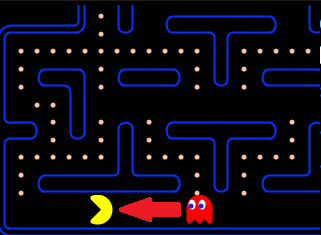
\includegraphics[scale=0.5]{D2.png}
\caption{ Chase Function }
\label{fig:Chase}
\end{figure}


\subsubsection{Scatter}
The scatter-mode will act as in the original pacman. The only change will be that it also would use the new A* Pathfinding system to find the corner that the ghost belongs to and create a patrol path that the ghost will follow.


\begin{figure}[!htbp]
\centering
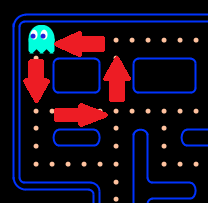
\includegraphics[scale=0.5]{D3.png}
\caption{ Scatter Function }
\label{fig:Scatter}
\end{figure}


\subsubsection{Random and Frightened}
The random and frightened mode will both use the same movement system. When a ghost meets an intersection in the maze it will then make a random decision about which way to go. Obviously the ghost won’t be allowed to move back in the direction which it came. In frightened mode the ghost keeps the same system but will also keep in mind where in the maze pacman is located and try to avoid going in direction which pacman is located.


\begin{figure}[!htbp]
\centering
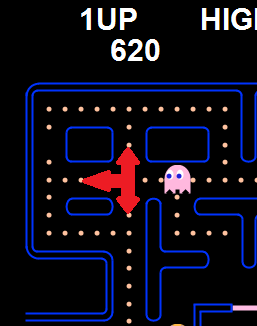
\includegraphics[scale=0.5]{D4.png}
\caption{ Random Function }
\label{fig:Random}
\end{figure}

\begin{figure}[!htbp]
\centering
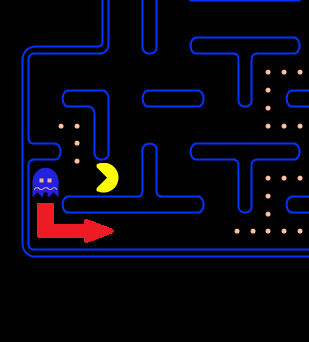
\includegraphics[scale=0.5]{D5.png}
\caption{ Frightened Function }
\label{fig:Frightened}
\end{figure}

\subsubsection{A* Pathfinder}
As mentioned before an A* Pathfinder will be the pathfinder choice, this will replace the calculation the ghosts make each intersection in the maze and replace it with a system that always tracks the fastest way to pacman.

The A* Pathfinder work as following:

As seen on A* Fig (1) a grid is applied over the game maze. Since the original pacman also is a grid based game this implementation will be good match for the game. The grid is informed about which coordinates that are able to be used as a path. These coordinates will be marked as true, and the rest, which in our case are walls, will be marked as false. A start point, in our case the ghost, and an end point which is pacman is being placed on the grid.


\begin{figure}[!htbp]
\centering
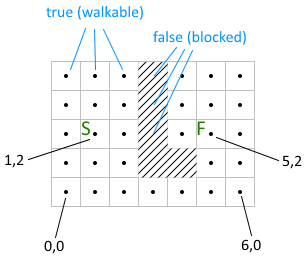
\includegraphics[scale=0.5]{D6.png}
\caption{ A* Part 1 }
\label{fig:A1}
\end{figure}

Every point in the grid has been giving three values which is F , G and H as seen in A* Fig (2). In this case a node is a set of coordinates.

G is the length of the path from the start node to the current point.
H is the distance from the current node and until the end point.
F is the total length of the route which it both the G and H added together.


\begin{figure}[!htbp]
\centering
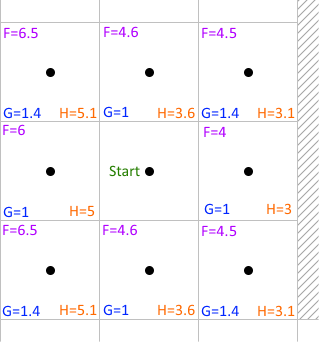
\includegraphics[scale=0.5]{D7.png}
\caption{  A* Part 2 }
\label{fig:A2}
\end{figure}


With these values given to the nodes the system is now ready to calculate the most optimal route to take. The system will value the nodes and put them in a list so they can be evaluated. The node with the lowest H value to be the fastest way to the end point. After a step is taken the node is being set as closed as can be seen on A* Fig (3) in order to make sure that the system won’t use the same node again.


\begin{figure}[!htbp]
\centering
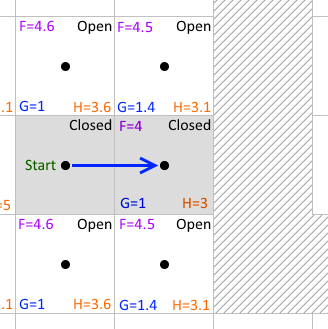
\includegraphics[scale=0.5]{D8.png}
\caption{  A* Part 3 }
\label{fig:A3}
\end{figure}


Another step in the process is to make sure the system also can calculate and find the fastest way through a diagonal path. In our case it won’t be needed since there is no diagonal paths to take in pacman.


\begin{figure}[!htbp]
\centering
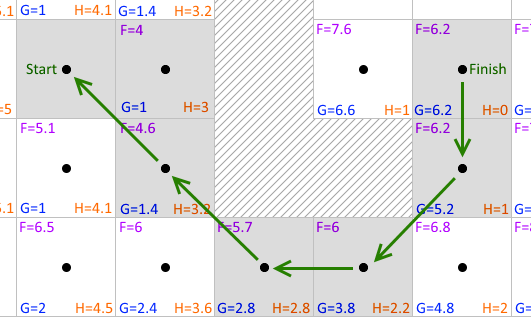
\includegraphics[scale=0.5]{D9.png}
\caption{  A* Part 4 }
\label{fig:A4}
\end{figure}


\subsubsection{Simulation}

Now that the game has its modes; mode cycle and pathfinding adapted to the genetic algorithm, it needs a way to send these informations into the system. A method could be a simulation that can simulate games based on information from a level completed by a player. During a game of pacman the coordinates of the players movements could be recorded and put into an array with timestamps that later can be played in the simulation and simulate the exact movements from the last game. The speed could then be increased to run faster simulations and by that increase the rate of information the genetic algorithm can receive. The information received by the genetic algorithm will be the simulation high score that can be used in the fitness function to calculate the most optimal simulation.


\subsection{Genetic Algorithm}

The information the GA receives is the players high-score and win/lose condition from the last played game. Our GA will be based on the research found in the analysis but before the algorithm is functional the GA variables from the list of requirements has to be fulfilled.


\subsubsection{Chromosomes}

Each chromosome serves as a single solution and in our case we want to find a way to optimize the modes for our ghosts. So each solution should contain a set of four genes of different sets of modes that combined should be able to make the game more challenging for the player playing with ghosts that has the next generation modes.

\subsubsection{Population Size}

The population size is based on the amount of simulation that our system can provide. According to our initial research a good population size is about 100. That means between the first generation and the second generation an amount of 100 simulations has to be played and analyzed before the next game of pacman can take place.


\subsubsection{Fitness function and Fitness Score}

The fitness function is going to be based on the simulation high scores. After the simulations has been played each simulation has been given a high score of how well pacman did in the current round. If pacman/player dies with a low highscore, it means that the ghosts have been very

successful and that chromosome then gets a high fitness score The simulations will be compared and the simulation that gave pacman the lowest high score will be the winner of that current generation.


\subsubsection{Selection}

Elitism
We are looking for a selection method that increases fast and keeps the best solutions and improves them. According to our research Elitism fulfill our requirements and priorities like this, Elitism always uses the best chromosomes or the single best according to what the setup is. This will increase the performance of the genetic algorithm rapidly.

\subsubsection{Crossover}
The crossover is based on our research and is being set to 80%

Single Point Crossover:
This method works by taking one small part of a chromosome A and swaps that into chromosome B and by that create a changed chromosome that can be tested once again (See fig. 1).


\begin{figure}[!htbp]
\centering
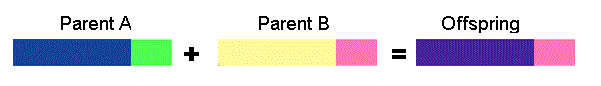
\includegraphics[scale=0.5]{D11.png}
\caption{ Single Point Crossover }
\label{fig:Crossover}
\end{figure}


\subsubsection{Mutation}
As mutation is there to create small random changes in the genes we want it to be low. This is the case since we want our chromosomes to be based on the simulations and not entirely by random mutations. We follow the recommendations from our research and place the mutation rate as 0.5%.

\subsection{UML}

\begin{figure}[!htbp]
\centering
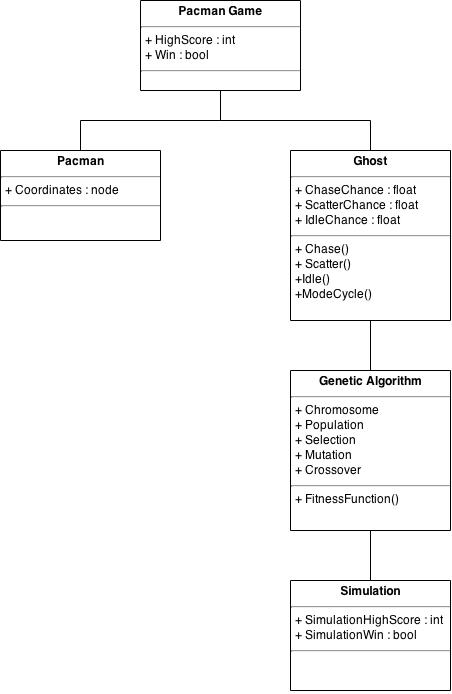
\includegraphics[scale=0.5]{D12.png}
\caption{ UML }
\label{fig:UML}
\end{figure}

\subsection{Summary}

The prototype should work as following:

\begin{enumerate}
\item A player plays a level of Pacman.

After the playthrough of the pacman level af set of coordinates of pacman is saved in an array and ready for the simulation to use.

\item The genetic algorithm creates new mode cycles that will be simulated

Based on the first generation chromosome the genetic algorithm will create new chromosomes that will be used in the new population.

\item The simulations use the player coordinates as input for simulating.

An amount of simulations is being played based on the population size and will generate a set of data for the fitness function to evaluate.

\item The simulations will be evaluated and the winning chromosome will be returned to the Pacman game.

\item The player will play a game with the new generation of ghost modes that should match the players performance.

\end{enumerate}


%!TEX root = ../main.tex

\section{Implementation} \label{sec:implementation}
For implementing our genetic algorithm we have used an open-source clone of pac-man made in C\# by Brian Bender~\footnote{Pac-man C\# implementation:~\url{https://www.planet-source-code.com/vb/scripts/ShowCode.asp?txtCodeId=5669&lngWId=10}}.

\subsection{Modes}
The open-source version of pac-man, which we are using as a base for the implementation, did not include ghost behaviour modes (XX see Design).
The ghosts do not actively chase pacman or scatter to individual corners as in the original pac-man.
They move by randomly selecting a point from a list of moveable points.

\begin{lstlisting}[caption=XXimage, label=lst:imp1]
if (currentMode == Cycle.MonsterMode.IsRandom) {
	ArrayList pts = GetNextPossibleCoordinates(_direction, _currentLocation);
	int iSelected = _rnd.Next(1, pts.Count + 1);
	Point SelectedPoint = (Point)pts[iSelected - 1];

	if (_currentLocation.Y < SelectedPoint.Y)
	_direction = CharacterDirection.Down;
	else if (_currentLocation.X < SelectedPoint.X)
	_direction = CharacterDirection.Right;
	else if (_currentLocation.X > SelectedPoint.X)
	_direction = CharacterDirection.Left;
	else if (_currentLocation.Y > SelectedPoint.Y)
	_direction = CharacterDirection.Up;

	MoveToEndPoint(_direction, GetDestinationCoordinate(_direction, _currentLocation));
}
\end{lstlisting}

As inspiration for movement patterns (aka modes) we referred to how the original pac-man moved the ghosts~\autocite{Mateas2003}.
These would become the ghost \emph{modes}.
The important thing was not to mimic pac-man exactly but rather to have different parameters for the ghosts behaviours to cycle through in the GA.

Although no modes or pathfinding was present in the source code, it did include methods for movement of the ghosts, \texttt{Move()}, and collision detection, \texttt{CanMove()}.
We used these pre-existing methods to do the actual movement of the ghosts, but in order to do \emph{chase} and \emph{scatter} we needed a pathfinding system.

\subsubsection*{pathfinding + neighbors}
Originally, an A* search algorithm was implemented (See appendix~\ref{sec:astar}) as a pathfinder, but it proved a hog on the system resources, so a much simpler method was created, inspired by the pathfinding of the original pac-man (See Analysis~\ref{ssub:pathfinding}).

The way pathfinding was done, four \emph{neighbors} were created one point left, right, below and above the ghost’s current location.

\begin{lstlisting}[caption=Neighbor class, label=lst:neighbor]
public class Neighbors
{
	int x;
	int y;
	private double distance;

	public int X
	{
		get { return x; }
		set { x = value; }
	}

	public int Y
	{
		get { return y; }
		set { y = value; }
	}

	public double Distance
	{
		get { return distance; }
		set { distance = value; }
	}
}
\end{lstlisting}

\begin{lstlisting}[caption=Instantiate neighbors, label=lst:instantiateneighbors]
//Create List<> to contain each neighbor of the ghost in question.
List<Neighbors> neighbors = new List<Neighbors>();

//Create four neighbors right, left, above and below the ghosts current location.
Neighbors rightNeighbor = new Neighbors() { X = currentLocation.X + 1, Y = currentLocation.Y };
Neighbors leftNeighbor = new Neighbors() { X = currentLocation.X - 1, Y = currentLocation.Y };
Neighbors aboveNeighbor = new Neighbors() { X = currentLocation.X, Y = currentLocation.Y + 1 };
Neighbors belowNeighbor = new Neighbors() { X = currentLocation.X, Y = currentLocation.Y - 1 };
\end{lstlisting}

Then a check was done to see if the ghost could move to the individual neighbor’s location.

\begin{lstlisting}[caption=canMove check, label=lst:canMove]
//If the ghost can move to the location of the neighbor and the ghosts current direction is not the opposite
//of the direction of the neighbor, add that neighbor to the neighbors List<>.
if (board.CanMove(new Point(rightNeighbor.X, rightNeighbor.Y)) && direction != CharacterDirection.Left)
neighbors.Add(rightNeighbor);
if (board.CanMove(new Point(leftNeighbor.X, leftNeighbor.Y)) && direction != CharacterDirection.Right)
neighbors.Add(leftNeighbor);
if (board.CanMove(new Point(aboveNeighbor.X, aboveNeighbor.Y)) && direction != CharacterDirection.Down)
neighbors.Add(aboveNeighbor);
if (board.CanMove(new Point(belowNeighbor.X, belowNeighbor.Y)) && direction != CharacterDirection.Up)
neighbors.Add(belowNeighbor);
\end{lstlisting}

If the neighbor’s location was moveable, the distance of that neighbor’s location and the location of pac-man, was calculated.

\begin{lstlisting}[caption=calculate distances,label=lst:distance]
//Create List<> to contain the distances of each neighbor to pac-man.
List<double> distances = new List<double>();

//Calculate distance from neighbors to pac-man.
foreach (Neighbors n in neighbors)
{
	n.Distance = Distance(new Point(n.X, n.Y), pacmanLocation);
	if (!distances.Contains(n.Distance))
	distances.Add(n.Distance);
}
\end{lstlisting}

\begin{lstlisting}[caption=Distance method,label=lst:distanceMethod]
//Calculate distance between passed Points. In this case the distance between each ghost neighbor and pac-man.
public double Distance(Point from, Point to)
{
	double a = from.X - to.X;
	double b = from.Y - to.Y;
	double distance = Math.Sqrt(a * a + b * b);
	return distance;
}
\end{lstlisting}

The neighbor with the shortest distance to pac-man would then determine the ghost’s next point to move to.

\begin{lstlisting}[caption=select point,label=lst:selectPoint]
//The neighbor (contained in neighbors List) which has the same distance as the first item
//in sorted List distances (shortest distance from pac-man), decides the point (relative to the ghost) which the ghost has to move to.
if (neighbors.Contains(rightNeighbor) && rightNeighbor.Distance == distances[0])
go = new Point(1, 0);

else if (neighbors.Contains(leftNeighbor) && leftNeighbor.Distance == distances[0])
go = new Point(-1, 0);

else if (neighbors.Contains(aboveNeighbor) && aboveNeighbor.Distance == distances[0])
go = new Point(0, 1);

else if (neighbors.Contains(belowNeighbor) && belowNeighbor.Distance == distances[0])
go = new Point(0, -1);

//return the point closest to pac-man which the ghost can move to.
return go;

\end{lstlisting}

The ghosts only check for a new move location and direction at every intersection in the game level, and so a method was created to generate a lists of the location of every intersection.

\begin{lstlisting}[caption=generate intersections,label=intersections]
//Generate HashSet<> which contains every intersection in the current level.
public void GenerateIntersections()
{
	intersections = new HashSet<Point>();

	intersections.Add(new Point(23, 26));
	intersections.Add(new Point(199, 26));
	intersections.Add(new Point(246, 26));
	intersections.Add(new Point(422, 26));
	intersections.Add(new Point(23, 97));
	intersections.Add(new Point(422, 97));
	intersections.Add(new Point(23, 150));
	intersections.Add(new Point(103, 150));
	intersections.Add(new Point(103, 256));
	intersections.Add(new Point(342, 256));
	intersections.Add(new Point(103, 97));
	intersections.Add(new Point(342, 97));

\end{lstlisting}

A foreach loop would check if the ghost’s location was equal to an intersection, and if so, pass the returned point from the Pathfinder method as the selected point to move towards.

\begin{lstlisting}[caption=pathfinder call,label=lst:pathfinderCall]
if (Pathfinder.Intersections.Contains(_currentLocation))
{
	go = pathfinder.ClosestNeighbor(_currentLocation, pacmanCurrentLocation, _board, _direction);
}

SelectedPoint = new Point(_currentLocation.X + go.X, _currentLocation.Y + go.Y);

if (_currentLocation.Y < SelectedPoint.Y)
_direction = CharacterDirection.Down;
else if (_currentLocation.X < SelectedPoint.X)
_direction = CharacterDirection.Right;
else if (_currentLocation.X > SelectedPoint.X)
_direction = CharacterDirection.Left;
else if (_currentLocation.Y > SelectedPoint.Y)
_direction = CharacterDirection.Up;

MoveToEndPoint(_direction, GetDestinationCoordinate(_direction, _currentLocation));
\end{lstlisting}

\subsection{Modes and Cycle}\label{ssec:modesCycle}
The \emph{GhostCharacter} class contains a Method called \emph{MoveMonster()}. What this method does is it moves the monster one time per frame, depending on what current mode is set for that ghost. The mode is controlled by a private variable called \emph{currentMode}. This is of the type \emph{MonsterMode} which is a custom enumerator, which is defined by the \emph{Cycle} class as described later. In the original source code, this method was used to move the ghosts randomly, and to animate them as well.

In order to make the ghosts move according to their \emph{MonsterMode}, we expanded the method with if statements as such:
\begin{lstlisting}
if (currentMode == Cycle.MonsterMode.IsRandom) {
\end{lstlisting}

This will instead make the ghost move according to their \emph{MonsterMode}, as described in the previous chapter.

The same is true of the MonsterModes \emph{IsChasing} and \emph{IsScattering}.

\subsubsection*{The Cycle}
Now we know that in order to make our ghosts move independently, we simply need to change their current MonsterMode. The idea of the cycle is that each ghost will independently have their MonsterMode changed, according to whatever parameters we (or the Genetic Algorithm) give them. This is where the custom made Cycle class comes in handy.

\begin{lstlisting}[caption=Cycle class and its constructor,label=lst:cycle]
using System;
using System.Collections.Generic;
using System.Linq;
using System.Text;

namespace Chomp
{
	[Serializable]
	public class Cycle
	{
		public enum MonsterMode
		{
			IsRandom = 0,
			IsChasing = 1,
			IsScattering = 2,
			IsFleeing = 3
		}
		public Cycle(MonsterMode mode, double cyclevalue)
		{
			Mode = mode;
			CycleValue = cyclevalue;
		}

		public MonsterMode Mode { set; get; }
		public double CycleValue { set; get; }

	}
}
\end{lstlisting}

The \emph{Cycle} class is the basis we use to switch between the different ghost modes. In the \emph{GhostCharacter} class, we have a member which is a  \emph{List<T>} of 3 \emph{Cycles}, called \emph{cycle}.
It is essential that it is a List, due to the fact that we have three different modes to cycle between. Each Cycle in the list contains a Mode and a CycleValue. The Mode is the previously described MonsterMode, and the CycleValue is the duration of each Mode. The CycleValue can also be translated into percentage, so each List’s Cycles have a total CycleValue sum of 100.

The usage of this system is as follows:
\begin{lstlisting}[caption=Snippet of GameBoard.cs and Cycle instantiation,label=lst:cycleInst]
initialCycle = new Cycle(Cycle.MonsterMode.IsChasing, 33.3);
initialCycleList = new List<Cycle>();
initialCycleList.Add(initialCycle);
initialCycle = new Cycle(Cycle.MonsterMode.IsRandom, 33.3);
initialCycleList.Add(initialCycle);
initialCycle = new Cycle(Cycle.MonsterMode.IsScattering, 33.3);
initialCycleList.Add(initialCycle);
\end{lstlisting}

We create 3 cycles each with a unique mode, and a total sum of 100, and add them each to our List. This List can then be applied to any ghost and it will follow the respective cycle, which in turn also is the way we apply it for the initial playthrough for the prototype, where initial playthrough in this case means the first time a test person plays the game.

This all comes together in the GameBoard class, where we call the method \emph{UpdateCycle()} on each frame for each ghost.

\begin{lstlisting}[caption=Snippet of GameBoard.cs showing the system to Cycle between modes for ghosts, label=lst:cycleModes]
public void UpdateCycle(GhostCharacter g)
{

	if (g.CycleUpdaterInternal >= 50 && g.CurrentInvinsibility != CharacterInvincibility.Vulnerable)
	{
		if (g.CurrentModeValue == 0)
		{
			if (g.CurrentCycle[0].CycleValue * 10 <= cycleUpdaterBigFrame)
			{
				Console.WriteLine("Switching to 1 from " + g.CurrentMode);
				g.CurrentMode = g.CurrentCycle[1].Mode;
				g.CurrentModeValue = 1;
			}
		}
		else if (g.CurrentModeValue == 1)
		{
			double t = 10 * g.CurrentCycle[0].CycleValue;
			if (t + g.CurrentCycle[1].CycleValue * 10 <= cycleUpdaterBigFrame)
			{
				Console.WriteLine("Switching to 1 from " + g.CurrentMode);
				g.CurrentMode = g.CurrentCycle[2].Mode;
				g.CurrentModeValue = 2;
			}
		}
		else if (g.CurrentModeValue == 2)
		{
			if (cycleUpdaterBigFrame >= 1000)
			{
				Console.WriteLine("Switching to 0 from" + g.CurrentMode);
				g.CurrentMode = g.CurrentCycle[0].Mode;
				g.CurrentModeValue = 0;
				cycleUpdaterBigFrame = 0;
			}

		}
		g.CycleUpdaterInternal = 0;
	}
	g.CycleUpdaterInternal++;
}
\end{lstlisting}

The method takes a GhostCharacter as input. The \emph{cycleUpdaterBigFrame} is an integer that runs from 0 to 1000, counting each frame. Depending on this, and a couple of other checks to ensure that the cycle is running accurately, it will change the MonsterMode of the individual ghost and reset the integer to reset the cycle. Using 1000 and multiplying by 10 is how we get the \emph{CycleValue} double to represent percentage.

the \emph{CycleUpdaterInternal} integer is in place to avoid running through the check on every frame, but only checks once per 50 frames for each ghost, which corresponds to about 1 second per check when playing the prototype in real time, since it is timed to run at one frame per 20 milliseconds during normal play.

This concludes how we control the behaviour for each ghost individually, how the different modes work, and how we switch between the modes.

\subsection{Flow}
\subsubsection*{Initial playthrough}
Before we move into the Genetic Algorithm part of the prototype, we will go over the flow of how the prototype progresses.

The Pac-Man clone is made in Windows Forms, so the initial startup of the application simply generates the form and it’s parameters, which can all be found in the frmScreen class. We’ve added additional variables and modified some values from the original to fit our needs better, such as changing the lives to 1 instead of 3, and adding a \emph{List<CharacterDirection>} member to record the player’s movement.

\begin{lstlisting}[caption=Snippet of frmScreen.cs taken from the key event handler, label=lst:keyEvent]
else if (e.KeyCode == Keys.F1)
{
	if (_board.Player2.GameOver)
	{
		GeneticStuff = new GA();
		GeneticStuff.InitializeGA();
		recordDirection.Clear();
		_board.CurrentPlayer.Score = 0;
		recording = true;
		recordTicker = 0;
		this.tmrMove.Interval = 20;
		this.microTimer.Enabled = false;

		StartGame(1);
\end{lstlisting}

The gameplay is started by pressing F1 on the initial splash screen.
Controlled by the key event handler frmScreen\_Keydown, this will call StartGame(1), instantiate the GA
 class for later use, as well as adjusting settings for playing the game and not simulating.

In StartGame(),  the GameBoard and characters (Pac-Man and ghosts) are instantiated. The last thing that happens in this method is the timer being started. The timer is of the type Windows.Forms.Timer and is set to run at an interval of 20 milliseconds. This begins the game.

The game advances by using the tmrMove\_Tick() event method, which is triggered at the interval of the Windows.Forms.Timer.

\begin{lstlisting}[caption=Snippet of frmScreen. A method called at each timer interval, label=lst:timerInterval]
private void tmrMove_Tick(object sender, System.EventArgs e)
{
	if (powerMode)
	{
		if (powerTicker > 90)
		{
			tmrPowerMode_Tick();
		}

		powerTicker++;

	}
	if (recording)
	{
		recordDirection.Add(_board.PacMan.AttemptedDirection);
		recordTicker++;
		_board.MoveCharacters();
		picGameBoard.Invalidate();
	}

	else if (!recording && normalPlayback)
	{
		if (recordTicker > playbackTicker)
		{
			_board.PacMan.AttemptedDirection = recordDirection[playbackTicker];
			playbackTicker++;
		}
		_board.MoveCharacters();
		picGameBoard.Invalidate();
	}
}

\end{lstlisting}

This method controls a few different things. As we need to run the game at a much faster speed when simulating, it was not appropriate to use a timer solution for triggering the state of the ghosts’ vulnerability, so this has been changed to be controlled by counting frames. If the boolean recording is true, it will record the players direction per frame and add it to the previously mentioned list. It will then call the MoveCharacters() method of the GameBoard class.

\begin{lstlisting}[caption=Snippet of GameBoard.cs. Method used to move and check collision for each character.,label=lst:collision]
public void MoveCharacters()
{
	UpdateCycle(_ghostRed);
	UpdateCycle(_ghostBlue);
	UpdateCycle(_ghostPink);
	UpdateCycle(_ghostYellow);
	_pacMan.Move();
	_ghostRed.MoveMonster();
	_ghostPink.MoveMonster();
	_ghostBlue.MoveMonster();
	_ghostYellow.MoveMonster();
	cycleUpdaterBigFrame++;

	GameCharacter g = PlayerCollided(_pacMan, _ghostRed, _ghostPink, _ghostBlue, _ghostYellow);

	if ( g != null)
	{
		Console.WriteLine(g);
		if (g.CurrentInvinsibility == CharacterInvincibility.Vulnerable)
		{
			g.Visible = false;
			_pacMan.Visible = false;
			_currentPlayer.Score += _currentEatScore;
			UpdateScore();
			if (frmScreen.recording)
			{
				_picGameBoard.Refresh();
				PaintEatScore(new Point(g.CurrentLocation.X - 15, g.CurrentLocation.Y - 10), Graphics.FromHwnd(_picGameBoard.Handle));
			}
			_currentEatScore *= 2;
			_pacMan.Visible = true;
			ResetMonster(g);
			if (frmScreen.recording)
			_picGameBoard.Refresh();

\end{lstlisting}

We already know what UpdateCycle() and MoveMonster() has do, as it is explained in~\ref{ssec:modesCycle} Move() is responsible for moving pacman depending on his current CharacterDirection.

The rest of this method is responsible for the collision detection. If Pac-Man and any of the ghosts collide with each other, the player’s turn will either end, or he will eat the ghost he collided with, depending on the ghost’s vulnerability status.

The following flow chart (figure~\ref{fig:imp1}) helps visualize the process of the initial playthrough:

\begin{figure}[!htbp]
	\centering
	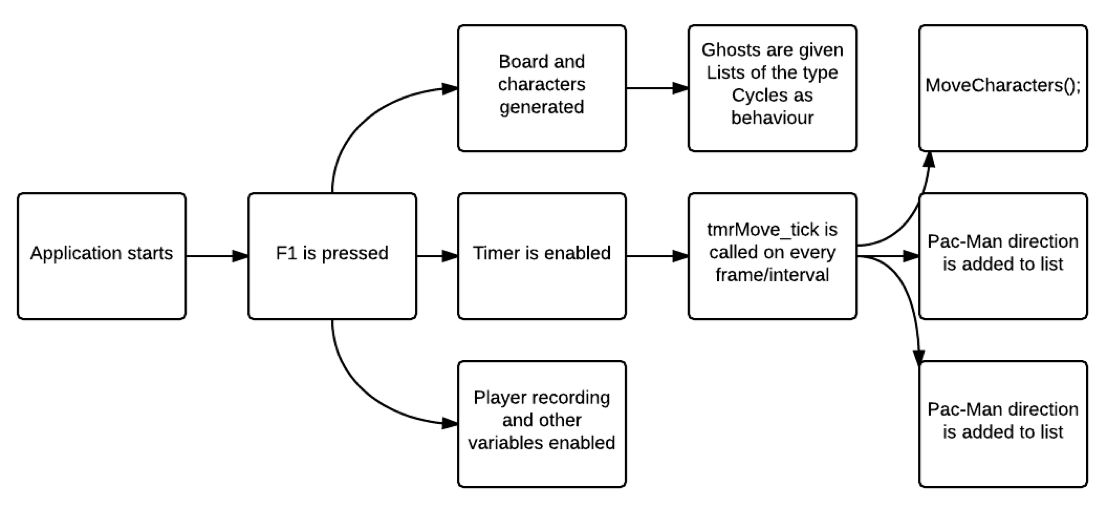
\includegraphics[width=0.95\textwidth]{imp_1.png}
	\caption{Flow of normal gameplay}
	\label{fig:imp1}
\end{figure}

\subsubsection*{Simulation}
The flow for simulations are fairly similar to initial playthrough.

\subsubsection*{Timer while simulating}
Instead of the timer being set to 20 ms, we gave it a value of 1 ms instead and tried running simulations with this. It was later discovered that the Windows.Forms.Timer has internal limitations, that prevent it from running faster than around 14 ms. This was very clear as simulations were not running much faster than when playing the game at normal spear.

This led us to trying to find a different way than using a Forms timer, and the first solution we tried implementing was running a continuous while loop, that would only end if the player died or won the game.

However, this also caused some problems. During testing with this implementation, we discovered that collision detection was nowhere near fast enough to keep up with the while loop, as the while loop would move the characters as fast as the CPU can handle, not allowing the collision detection of the game to react in time.

We attempted many different solutions to counteract this problem, such as creating async functions that would wait for each other, delaying the while loop substantially by making it process fake data, and trying to improve the Pac-Man clone’s collision detection.

Ultimately, we ended up not being able to use a while loop, and instead we came up with the solution of using the System.Diagnostics.Stopwatch as a timer instead. This Stopwatch class is not intended to be used as a timer, but we found a wrapper which allows it to be, by creating a subclass that uses the Stopwatch, allowing us to instantiate an extremely fast timer~\footnote{\url{http://www.codeproject.com/Articles/98346/Microsecond-and-Millisecond-NET-Timer}}. Since we did not need precision, but rather speed, it was not a problem if the timer was not accurate to the nanosecond.

Simulating with this timer had good results, as the game’s logic and collision detection was able to keep up. Testing at 0.5 ms sometimes lead to graphical glitches, as the GameBoard is refreshed on every frame. When this happens the game is unable to recover, and collision is broken for the rest of the time the application is run. The timer ended up being set to about 1.8 ms, which allowed us to have reasonably fast simulations and also keep collision detection.

\subsubsection*{Playback}
As mentioned before, the player’s CharacterDirection is recorded every frame, which allows us to run through this recording, and play it back once per frame accordingly. Since there are no physics involved, the playback will always match the input of the player.

\begin{lstlisting}[caption=Snippet of frmScreen.cs. High resolution timer event method, label=lst:timer]
private void moveTick_while(object sender, MicroTimerEventArgs timerEventArgs)
{
	if (powerMode)
	{
		if (powerTicker > 90)
		{
			tmrPowerMode_Tick();
		}
		powerTicker++;
	}
	if (recordTicker > playbackTicker)
	{
		_board.PacMan.AttemptedDirection = recordDirection[playbackTicker];
		playbackTicker++;
		_board.MoveCharacters();
		picGameBoard.Invalidate();
	}
	if (recordTicker <= playbackTicker)
	{
		_board.MoveCharacters();
		picGameBoard.Invalidate();
	}
}
\end{lstlisting}

On each frame, we run a check on whether or not the playback frame is smaller than the recorded frame, and if it is, we will set Pac-Man’s direction to the matching direction on the frame it was recorded. If however there is nothing more to play back, the game will still as before, but Pac-Man will no longer move. A case for this could be where the player died very quickly, but on the simulation the ghosts will have a different behaviour, making them reach Pac-Man at a later time.

\subsection{Genetic Algorithm}
\subsubsection*{Framework}
For implementing a Genetic Algorithm to handle our calculations, we have chosen to use the Genetic Algorithm Framework (GAF) for .NET 4 and 4.5~\footnote{\url{http://aiframeworks.net/}}.
The framework is easily available through the NuGet package manager, and can be installed using Visual Studio’s console.

As inspiration for our own implementation, we took a close look at their example for “The Travelling Salesman”, and how they have gone about solving it~\footnote{\url{http://aiframeworks.net/blog/gaf-part-4}}.

This framework allows us to use objects as genes, which is perfect as we can cast them into the List of Cycles that we need for each ghost. The chromosomes are supposed to be a solution for each time we run a simulation, which means the chromosome needs to be created of 4 different genes, one gene for each ghost. According to previous research (~\ref{ssub:population}, a decent sized population ranges from 20 to 100, so we have decided to go with 20 chromosomes per generation for our prototype.

\subsubsection*{Gene creation (first generation)}
As mentioned before, each ghost must have a List of Cycles in order to control their behaviour. Our initial gene creation creates completely random genes for each ghost. These are then collected and added to a single gene. Twenty of these make up our population.

\begin{lstlisting}[caption=Snippet of GA.cs. Gene creation method, label=lst:genes]
private List<Cycle> CalculateGenes()
{
	List<Cycle> gene = new List<Cycle>();

	Cycle cycle1;
	Cycle cycle2;
	Cycle cycle3;

	//Random rnd = new Random();
	int r;

	double alpha = 0, beta = 0, gamma = 0, k = 0;

	alpha = rnd.Next(0, 100);
	beta = rnd.Next(0, 100);
	gamma = rnd.Next(0, 100);

	k = (alpha + beta + gamma) / 100;

	alpha /= k;
	beta /= k;
	gamma /= k;

	List<Cycle.MonsterMode> monsterList = new List<Cycle.MonsterMode>();
	monsterList.Add(Cycle.MonsterMode.IsRandom);
	monsterList.Add(Cycle.MonsterMode.IsChasing);
	monsterList.Add(Cycle.MonsterMode.IsScattering);

	r = rnd.Next(monsterList.Count);
	cycle1 = new Cycle(monsterList[r], alpha);
	monsterList.Remove(monsterList[r]);

	r = rnd.Next(monsterList.Count);
	cycle2 = new Cycle(monsterList[r], beta);
	monsterList.Remove(monsterList[r]);
	r = rnd.Next(monsterList.Count);
	cycle3 = new Cycle(monsterList[r], gamma);
	monsterList.Remove(monsterList[r]);

	gene.Add(cycle1);
	gene.Add(cycle2);
	gene.Add(cycle3);

	return gene;
}
\end{lstlisting}

The List of Cycles is first created, then populated with random values that have a total sum of 100, and a random MonsterMode. This process is repeated 4 times for each chromosome.

\begin{lstlisting}[caption=Snippet of GA.cs. Adding genes to chromosomes, label=lst:geneChromosome]
population = new Population(20); // Amount of simulations
ghostChromosomes = new List<List<Cycle>>();
//Fill our population with chromosomes, which each contain 4 genes.
for (int p = 0; p < 10; p++)
{
	ghosts = new List<List<Cycle>>();
	ghosts = CreateGhosts();
	Chromosome chromosome = new Chromosome();
	for (int h = 0; h <= 3; h++)
	{
		chromosome.Genes.Add(new Gene(ghosts[h]));

	}
	population.Solutions.Add(chromosome);
}
\end{lstlisting}

\subsubsection*{Simulations using the Genetic Algorithm}
We create our population and fill it with the chromosomes generated by the previous method. When the game simulates, we give each ghost one of our created genes, from the list of chromosomes. This is done as such:

\begin{lstlisting}[caption=Snippet of frmScreen.cs. Key event handler starting the simulation, label=lst:keyHandler]
else if (e.KeyCode == Keys.F9)
{
	runNumber++;
	tmrBlink.Enabled = true;
	var t = GeneticStuff.FittestPerGeneration;
	_board.Blinky.CurrentCycle = (List<Cycle>)t.Genes[0].ObjectValue;
	_board.Inky.CurrentCycle = (List<Cycle>)t.Genes[1].ObjectValue;
	_board.Pinky.CurrentCycle = (List<Cycle>)t.Genes[2].ObjectValue;
	_board.Clyde.CurrentCycle = (List<Cycle>)t.Genes[3].ObjectValue;
	_board.Blinky.CurrentMode = _board.Blinky.CurrentCycle[0].Mode;
	_board.Inky.CurrentMode = _board.Inky.CurrentCycle[0].Mode;
	_board.Pinky.CurrentMode = _board.Pinky.CurrentCycle[0].Mode;
	_board.Clyde.CurrentMode = _board.Clyde.CurrentCycle[0].Mode;
	Console.WriteLine(_board.Blinky.CurrentCycle[0].Mode + " " + _board.Inky.CurrentCycle[0].Mode + " " + _board.Pinky.CurrentCycle[0].Mode + " " + _board.Clyde.CurrentCycle[0].Mode);

	recordDirection.Clear();
	_board.CurrentPlayer.Score = 0;
	recording = true;
	recordTicker = 0;
	this.tmrMove.Interval = 20;
	this.microTimer.Enabled = false;

	StartGame(1);
}
\end{lstlisting}

We cast each gene to a List of Cycles, and assign them to our ghost. We then set the mode of each ghost to be the first mode in it’s newly given List of Cycles. We then set the score to 0 and start our high resolution timer, in order to evaluate the proposed solution.

This is only for the first simulation in a generation. We have automated the process to evaluate the rest of the chromosomes in the population as well.

If Pac-Man is killed or is successful in eating all the pellets, UpdateChromosome() is called.

\begin{lstlisting}[caption=Snippet of frmScreen.cs. UpdateChromosome method to change chromosome for each simulation, label=lst:updateChromosome]
private void UpdateChromosome(int s, bool w=false)
{
	Logger previousRun = new Logger();
	previousRun.Score = s;
	previousRun.LoggedChromosome = GeneticStuff.population.Solutions[currentChromosome-1];
	Console.WriteLine(GeneticStuff.population.Solutions[currentChromosome - 1].Id);
	previousRun.WinLoss = w;
	currentRunLog.Add(previousRun);

	if (currentChromosome < GeneticStuff.population.Solutions.Count)
	{
		_board.CycleUpdaterBigFrame = 0;
		int t = currentChromosome;

		_board.Blinky.CurrentCycle = (List<Cycle>)GeneticStuff.population.Solutions[t].Genes[0].ObjectValue;
		_board.Inky.CurrentCycle = (List<Cycle>)GeneticStuff.population.Solutions[t].Genes[1].ObjectValue;
		_board.Pinky.CurrentCycle = (List<Cycle>)GeneticStuff.population.Solutions[t].Genes[2].ObjectValue;
		_board.Clyde.CurrentCycle = (List<Cycle>)GeneticStuff.population.Solutions[t].Genes[3].ObjectValue;
		_board.Blinky.CurrentMode = _board.Blinky.CurrentCycle[0].Mode;
		_board.Inky.CurrentMode = _board.Inky.CurrentCycle[0].Mode;
		_board.Pinky.CurrentMode = _board.Pinky.CurrentCycle[0].Mode;
		_board.Clyde.CurrentMode = _board.Clyde.CurrentCycle[0].Mode;
		SimulationFast();
		Console.WriteLine(currentChromosome);
		Console.WriteLine(s);

	}
\end{lstlisting}

UpdateChromosome() takes 2 arguments, an int representing the score for the simulation and a boolean representing whether or not the simulation won. For this purpose we have created another custom Class, which we use as a type to log data for each of the simulations. We store the score, the ID for the respective chromosome, as well as whether or not the player won.

We then make a check if there are more chromosomes left in the current population to run through, and if so we give the ghosts the next List of Cycles, or genes, and run the simulation again.

Once there are no more simulations, we call on the GA to evaluate the simulations and assign them a fitness score.


\begin{lstlisting}[caption=Snippet of frmScreen.cs continued. Starting the GA and evaluation, label=lst:gaEvo]
microTimer.Enabled = false;
Console.WriteLine("done simulating");
ga = new GeneticAlgorithm(GeneticStuff.population, CalculateFitness);
int c = 0;
foreach (object o in currentRunLog)
{
	//Console.WriteLine(currentRunLog[c].LoggedChromosome.Id + " " + ga.Population.Solutions[c].Id);
	c++;

}
ga.OnGenerationComplete += GeneticStuff.ga_OnGenerationComplete;
ga.OnRunComplete += GeneticStuff.ga_OnRunComplete;
ga.Operators.Add(GeneticStuff.elite);
ga.Operators.Add(GeneticStuff.crossover);
ga.Operators.Add(GeneticStuff.mutate);
if (runNumber > 0)
{
	foreach (Chromosome p in ga.Population.Solutions)
	{
		p.Evaluate(CalculateFitness);
	}
}
ga.Run(Terminate);
\end{lstlisting}

We instantiate the GeneticAlgorithm(GA) type which is defined by the GAF. This takes a population and a method for calculating fitness as arguments.
We then subscribe to our event handlers, and add our operators to the Genetic Algorithm.

We then tell the algorithm to start, with Terminate as the method for when it should stop. In our case, the Terminate is set to stop after two generations, because we can only give it the score of each simulation for one generation at a time.

However, allowing it to run for two generations lets the GA first evaluate the score for each simulation, and then create a new population based on the results of this. This has the backwards effect of giving all the chromosomes in the second generation a fitness value of 1, as our fitness function will always return 0 as score.

In order to solve this problem, we implement a check to check what generation we are currently evaluating. If this is above 0, then it will force a re-evaluation of all the chromosomes in a population. As we store the chromosome IDs in the List of Loggers, we can always match a simulation and chromosome to each other, which makes this re-evaluation possible.

\subsubsection*{Fitness Function}
Our fitness function works quite simply by checking what the final score was for a simulation. The chromosome is given a fitness level based on this.

\begin{lstlisting}[caption=snippet of frmScreen.cs. Methods to calculate fitness for each chromosome., label=lst:fitness]
public double CalculateFitness(Chromosome chromosome)
{
	double min = 3000;
	double score = 1-(GetScoreFromRun(chromosome)/ min);
	return score;
}
public int GetScoreFromRun(Chromosome chromosome)
{
	int c = 0;
	int q = 0;
	Console.WriteLine(chromosome.Id);
	if (chromosome != null)
	{
		foreach (object o in currentRunLog)
		{
			if (chromosome.Fitness == 1 && currentRunLog[c].LoggedChromosome.Id == chromosome.Id)
			{
				Console.WriteLine("something went wrong");
			}
			if (currentRunLog[c].LoggedChromosome.Id == chromosome.Id)
			{
				q = currentRunLog[c].Score;
				Console.WriteLine(currentRunLog[c].LoggedChromosome.Id + " " + chromosome.Id);

			}
			c++;
		}
	}
	return q;
}
\end{lstlisting}

In the first edition of the prototype, the worst case scenario for the ghosts are that Pac-Man gets a score of 3000. This will later be revised through pre-testing, finding a more optimal value to evaluate against.
For each chromosome that runs through the CalculateFitness() method, GetScoreFromRun() is also called. In this method, we match the chromosome given as argument against a logged chromosome, using the unique ID string that GAF gives it. This also means that if the chromosome can’t be matched to a logged simulation, it will return a score of 0, giving the chromosome the best possible evaluation. This is why we need to re-evaluate once the simulations have actually been run, as mentioned before.

\subsubsection*{Logger class}
\begin{lstlisting}[caption=Logger class and its constructor.,label=lst:logger]
namespace Chomp
{
	[Serializable]
	public class Logger
	{
		public Logger()
		{
			WinLoss = false;
		}

		public int Score { set; get; }
		public bool WinLoss { set; get; }
		public Chromosome LoggedChromosome { set; get; }
	}
}
\end{lstlisting}

For each simulation we store a Logger object in a List. This is simply to keep track of the runs and to be sure that the evaluated chromosome matches the chromosome for that particular simulation.

As we store a Chromosome object in each Logger, we can directly match it using the unique ID-string given by the GAF.

\subsubsection*{Genetic Algorithm Operators}
Some operators are pre-made and come as part of the GAF. Although it is a possibility to create your own operators, our research indicates that the operators included will suit our needsXXREF.The operators that we have in use are Elite~\footnote{\url{http://aiframeworks.net/microsites/gaf/html/9a476085-c561-dc6d-f30e-69e720795e1c.htm}}, SwapMutate~\footnote{\url{http://aiframeworks.net/microsites/gaf/html/7677aa9e-d365-3e26-cf64-376f994b1f45.htm}} and CrossOver~\footnote{\url{http://aiframeworks.net/microsites/gaf/html/49d4e899-e9a0-473e-815a-e2b3a35d2465.htm}}

The parameters chosen for each operator are inspired by “The Travelling Salesman” example, and these values correspond with our research for each operator XXREF.


We have created a class diagram which shows the inheritance and interfacing between all the classes, to help give a better understanding of how the prototype is working. The class diagram can also be seen in expanded form in the appendix, where we have all the members of each class visible. XXRef til appendix

\begin{figure}[!htbp]
	\centering
	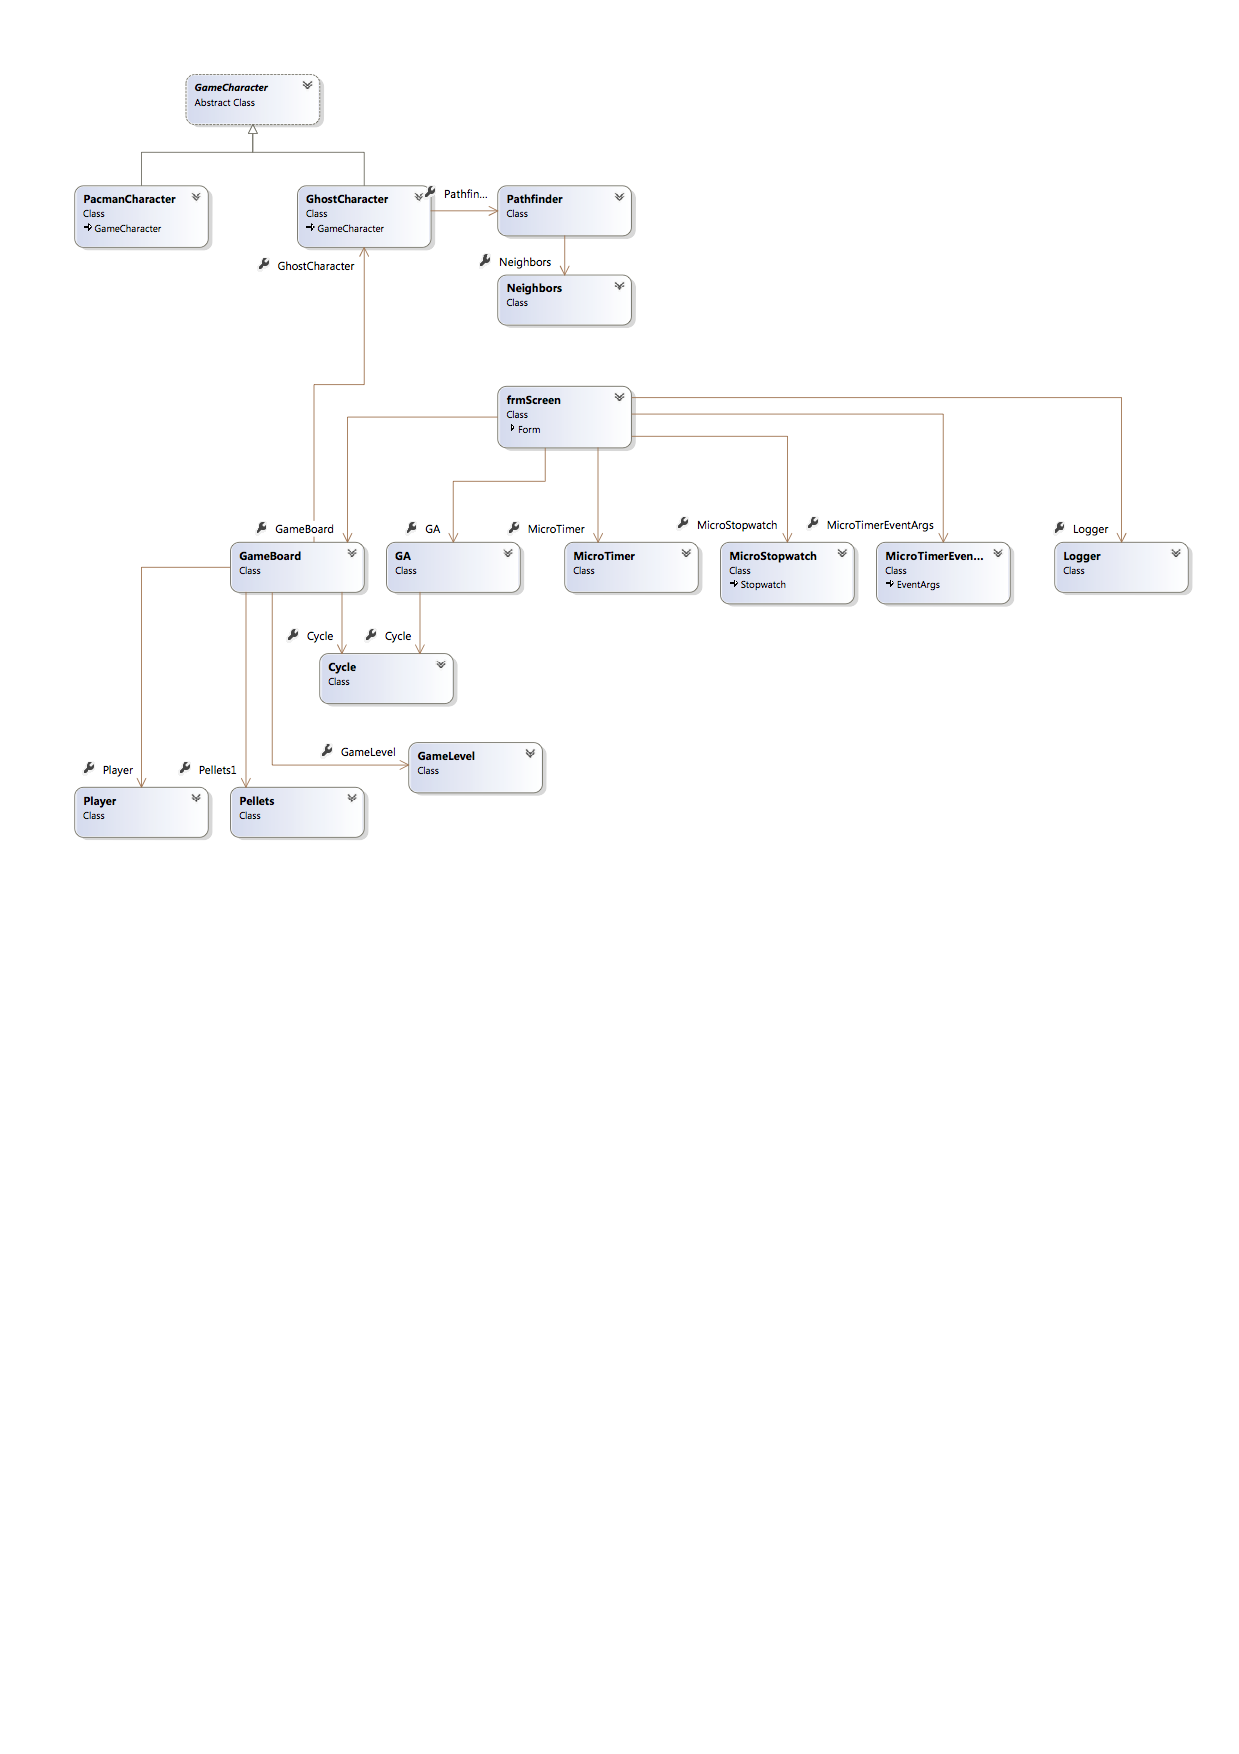
\includegraphics[width=1.00\textwidth]{ClassDiagram.png}
	\caption{Class diagram with inheritance and interfacing between the classes}
	\label{fig:class}
\end{figure}


\section{Evaluation} \label{sec:evaluation}
\section{Re-design} \label{sec:redesign}

This chapter is about using the knowledge gained from the discussion and then re-design the product to optimize it for the final problem statement.

\subsection{Pac-Man}


\subsubsection{Pacman Artificial Intelligence}

One of main reasons that we received random deaths from pac-man in the simulations were due to pacman dying at places where players normally would have avoided the ghosts. These deaths were caused by pacman stopping in the simulation at the point where the player died in the real game. There are also cases were pacman simply ran blindly into the ghosts during the simulation. The conclusion is that these actions could be removed by optimising pacman with an AI that could work as a player during simulations to reenact real game situation.  

This could be done by adding a new recording system for the simulator. Instead of tracking each of pac-man's coordinates, a system that tracks the players pattern could be made. This pattern recognition could work as following:

When the player makes his playthrough of the game the pattern recognition will take notes on how the player behaves throughout the maze. It will use these behaviors in the simulation to simulate like the player and instead of walking directly into a ghost, it might take the decision of turning in a direction that the player would have taken. This would challenge the GA  more and force it to create more challenging ghosts based on the fitness function.


\subsubsection{Frozen Ghosts}

The frightened mode encountered some bugs along the way that got the ghosts stuck in the maze. It got remade and was programed to make the ghosts freeze at the spot when pac-man entered the energizer mode. If the ghosts were lined up correctly the player could many of the ghosts and gain a higher score than intended. This could be a possible reason for the player points spikes in our data sets.


\subsubsection{Pacman Stuck}

When a player lost a game of pac-man and the simulation began running pac-man ended up with missing some paths to follow. This was caused by the way pac-mans movements were recorded by directions for each frame. In the simulation pac-man simply stopped changing directions at the frame that player died in the real game. This caused that any ghost with any set of modes could hit pac-man and might get a better evaluation score than deserved. 


Test participants missing feedback from the game

Some feedback that was given during testing was missing feedback from the game itself. One of the aspects were missing sound. Some of the test participants had a hard time to calculate how long pac-man would be in energized mode and sometime didn’t even realise that they had left the mode before running into a ghost. Another aspect were missing feedback on when the ghost changed behavior. Some of the participants found it unfair that the ghosts changed mode without any kind of warning.


\subsubsection{Pathfinder Bug?}

One of the bugs that have been noticed is that the ghosts lose all sense of intelligence when pac-man is standing still or they change behavior at a unfortunate point in the maze. We suspect it to be something with our pathfinder but it has not been determined yet. 



\subsection{Genetic Algotrithm}

\subsubsection{Player performance} 

We have decided to base our players performance on the high score of the simulation of the players movements. The fitness score only uses the high score of each simulation. It compares all of the current solutions and finds the simulation that forced pac-man to get the lowest score in the simulation. By doing this we force the genetic algorithm to only aim for making the game more difficult for the player. If we wanted to make an more overall player performance and try to match players skill level, the equation should be changed to keep a balanced difficulty. 

To fulfill these new requirements the fitness function have to be re-designed. The player high score from the non-simulated game should be the focus point in the fitness score. After the simulations has been executed they will each be compared with the player high score. The evaluation in the fitness function will work like this. The equation will pick the one simulations that is just below the player hight score and another simulation that is just above. From here it will detect if the player won or lost his last game. If the player has won his game the simulation that is slightly above the player high score will chosen as the new chromosome. If the player on the other hand has lost his game the simulation that is slightly below the player high score will be chosen as the new chromosome.

Player performance will be considered a match if the following occurrences is observed:

Test participants with different skill levels, will play defined amount of games where of each game represent a new generation. The obtained score must be the amount of points attained , as specified in a threshold. A threshold value of points in the prototype will be determined as well.
If the points obtained by the test participants are higher than the threshold - the genetic algorithm will adjust accordingly and increase the difficulty. Likewise , if the player attains a lesser amount of points than the specified threshold the difficulty will be lowered according, allowing the player to attain points equal to the specified threshold.

\section{Discussion} \label{sec:discussion}

The following content consist of discussions concerning the general procedure of developing a prototype and evaluation of such to ultimately answer to the final problem statement. We discuss if we are indeed able to answer to the final problem statement, and specifies further research areas.


The final problem reads:

Is it possible to create an implementation of a video game AI, which alternates between the various states of a finite state machine, to match the player's performance through the use of a genetic algorithm?



In order to successfully answer to the final problem statement, there are several aspects that must be described separately.

The matching of player performance is, with the current implementation, assessed by evaluating the attained amount of point of each test participant over each generation. We state the the player performance is matched if the test results show that point acquired in one level/generation does not exceed the previous level/generation played. Thus the point obtained in the proceeding level must be either similar or lower.
In the evaluation(See section \ref{sec:evaluation}), we find through the use of deltascores and points obtained by the test participants within each generation/level and visualisations of such data through boxplots, that there indeed are changes in the scores over several generations, both increasing and decreasing amount of points.

Thus by the definition of matching player performance we were unable to create an implementation of a video game AI, which alternates between the various states of a finite state machine, to match the player's performance through the use of a genetic algorithm.

We do however state in the FPS that we ask if it is indeed possible to do so. In order to make such claim, that it is indeed possible to create such implementation - there are several aspects that must be discussed.

\textbf{Matching player performance}

With the current method of assessing player performance, we are only evaluating whether or not the implemented genetic algorithm, in some manner, is somewhat able to keep the player points obtained in the proceeding levels played by the same test participant, equal to the previous attained points or lower.


theoretically, this method only implies that the genetic algorithm will try to decrease the player score as much as possible.

Thus if the implementation of the genetic algorithm was done accordingly with the following definition of matching player performance, we might have gotten other results that could be used to successfully answer to the final problem statement.

Player performance will be considered matched if:

A threshold value of desired attainable points will be determined.

Test participants,with a varying skill level, will after playing X games whereof each game represent a new generation, attain an equal score. The score must attained be the score as specified as the threshold.

 Thus if the points attained by the test participants are higher than the threshold, the genetic algorithm will aim to decrease the player score. However if the player obtain a lesser amount than the threshold, the genetic algorithm will aim to allow a rise in the point obtained up till the threshold.

 \textbf{Alternation between the various states of a finite state machine}

Also, to successfully answer to the final problem statement, our implemented prototype is utilizing some modified version of Pac-man, with some implemented modified modes and modified behaviours. The implemented states of a finite state machine is one single solution and does only represent a single implementation whereof the problem statement asks in general if it is indeed possible to implement to match the player performance.

Theoretically, if the prototype was successfully implemented and the alteration between the various states of the finite state machine was proven as efficient as possible, we would be able to identify whether or not the described alterations of the AI would actually be sufficient to match the player's performance. No such claim can be proven with the current prototype, as it only represents a single solution, with a single type of modified modes and behaviours which, additionally, was unable to match the current specified, matching of player performance.

\textbf{Genetic Algorithm}

In the genetic algorithm, as implemented into out prototype, there are several decisions and methods that represent only one single solution as a prototype to help answer to the FPS.

A genetic algorithm is developed in accordance with some problem definition. Thus the GA is utilized to find some set of solutions to the given problem. In our prototype, the problem definition is described as how the GA can decrease the amount of points that a player obtains in our modified version of Pac-man.  Also, the population size, gene encoding, fitness function and fitness score representation along with crossover, selection and mutation function along with the appropriate probabilities of such represents a single solution to how one might try to successfully answer to the FPS(See section \ref{ssub:components} for a list of genetic algorithm requirements.



\textbf{Final remarks}
Thus to elaborate upon the possibility of successfully answer to the final problem statement we are unable to claim that is is possible with our implementation and evaluation. Though, as this only represent a single type of solution, where some modifications might alter the results, we cannot state that is is not possible to create an implementation of a video game AI, which alternates between the various states of a finite state machine, to match the player's performance through the use of a genetic algorithm.


\section{Conclusion} \label{sec:conclusion}

\clearpage
%------------------------------------------------------------------------------
% BIBLIOGRAPHY
%------------------------------------------------------------------------------
\pagestyle{plain}
\label{bibliography}
\printbibliography[heading=bibintoc]

\clearpage
%------------------------------------------------------------------------------
% APPENDICES
%------------------------------------------------------------------------------
% once appendices are started we can't go back
% make sure this is the last include!!!
\appendix
\appendixpage
\addappheadtotoc
\noappendicestocpagenum

\section{A* Pathfinder}\label{sec:astar}
\includepdf[pages=-]{./appendices/AStarPathFinder.pdf}

\section{Questionnaire}\label{sec:question}
\includepdf[pages=-]{./appendices/Questionnaire.pdf}

\end{document}
